\documentclass[12pt,a4paper]{article}
\usepackage{ctex}
\usepackage{geometry}
\usepackage{graphicx}
\usepackage{listings}
\usepackage{xcolor}
\usepackage{hyperref}
\usepackage{float} % 让 figure/table 可以用 [H] 固定位置

\geometry{left=3cm,right=3cm,top=2.5cm,bottom=2.5cm}

% 代码样式
\lstset{
    language=Java,
    basicstyle=\ttfamily\small,
    keywordstyle=\color{blue}\bfseries,
    commentstyle=\color{green!50!black},
    stringstyle=\color{orange},
    showstringspaces=false,
    numbers=left,
    numberstyle=\tiny,
    breaklines=true,
    frame=single
}

\begin{document}

\begin{center}
    \heiti\zihao{2} 山东大学 · Java编程技术 · 实验报告 \\
    \vspace{1cm}
\end{center}

\begin{tabular}{rl}
    课程名称: & Java编程技术 \\
    实验名称: & 一个简单的控制台应用程序 \\
    专业班级: & 通信一班 \\
    学生学号: & 202300120317 \\
    学生姓名: & 陈都阳 \\
    实验时间: & 2025年9月16日 \\
\end{tabular}
\newpage
\vspace{1cm}

\section*{实验目的}
\begin{enumerate}
    \item 掌握安装 SDK 软件包、Eclipse 软件、EditPlus 编辑软件的方法。
    \item 掌握设置程序运行环境的方法。
    \item 掌握编写与运行程序的方法。
    \item 理解面向对象的编程思想。
\end{enumerate}

\section*{实验要求}
\begin{enumerate}
    \item 编写一个简单的控制台应用程序,该程序在命令行窗口输出两行文字:\\
    “Hello World!” 和 “We are students.”。
    \item 使用 Eclipse 编译运行,并截图实验结果。
    \item 使用命令行方式编译运行,并截图结果。
    \item 实验后回答相关思考问题。
\end{enumerate}

\section*{实验内容}

\subsection*{源代码}
\begin{figure}[H]
\centering
\begin{lstlisting}
// HelloWorld.java
public class HelloWorld {
    public static void main(String[] args) {
        System.out.println("Hello World!");
        System.out.println("We are students.");
    }
}
\end{lstlisting}
\caption{HelloWorld 源代码}
\end{figure}

\subsection*{实验过程与结果}

\begin{figure}[H]
\centering
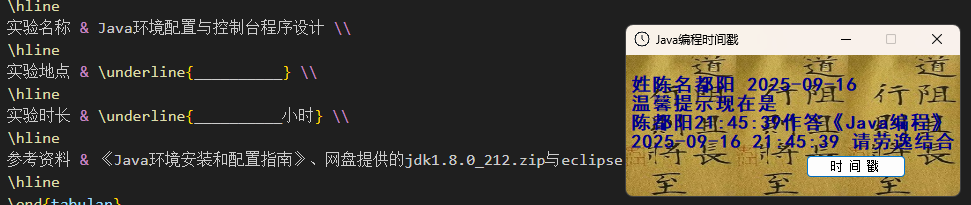
\includegraphics[width=0.8\textwidth]{eclipse_result.png}
\caption{Eclipse 运行结果}
\end{figure}

\begin{figure}[H]
\centering
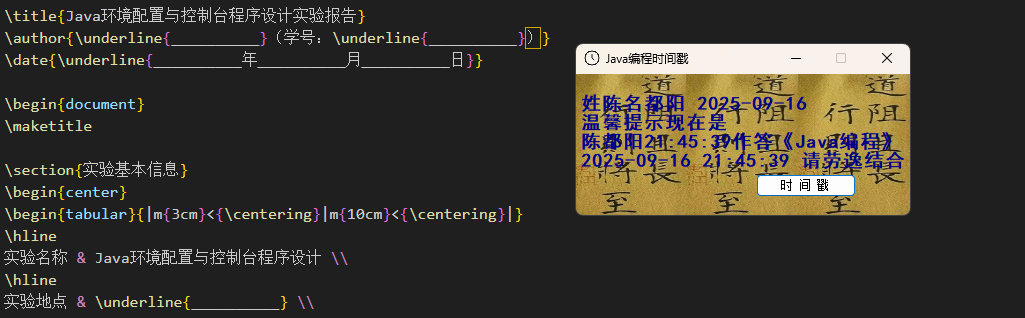
\includegraphics[width=0.8\textwidth]{cmd_result.png}
\caption{命令行运行结果}
\end{figure}

\section*{思考与分析}
\begin{enumerate}
    \item 编译器缺少大括号时,会提示 \texttt{'expected'} 错误。
    \item 编译器缺少分号时,会提示 \texttt{';' expected} 错误。
    \item 如果将 \texttt{System} 写成 \texttt{system},编译器会提示 \texttt{cannot find symbol}。
    \item 面向对象(OOP)是以对象为中心,强调对象之间的关系与交互;面向过程则是以步骤为中心,强调操作流程。  
    \item 例如五子棋:面向过程按步骤写函数(落子、判断输赢),面向对象则分为“玩家对象、棋盘对象、规则对象”,更模块化,扩展性更好。
\end{enumerate}

\section*{实验心得}
通过本次实验,我熟悉了 Java 开发环境的搭建,掌握了 Eclipse 和命令行编译运行 Java 程序的方法。同时,通过实验后的思考题,我加深了对面向对象与面向过程区别的理解。面向对象强调对象之间的协作,更适合大型系统的开发。

\end{document}
